\subsection{Virtual actuators and sensors} \label{chap: virtual}
Actuators and sensors are subject to various faults in the process. Due to these faults the system may experience drops in the performance which could lead to stability loss.

The objective of fault tolerant control using virtual actuators and sensors is to add a reconfiguration block which is presented as an extra layer between the faulty system and the controller, while the nominal controller is running. The purpose of the reconfiguration block in case of a fault is to provide fault tolerance by using the virtual actuators and sensors as can be seen in figure \ref{fig:VA}.

\begin{figure}[H]
	\centering
	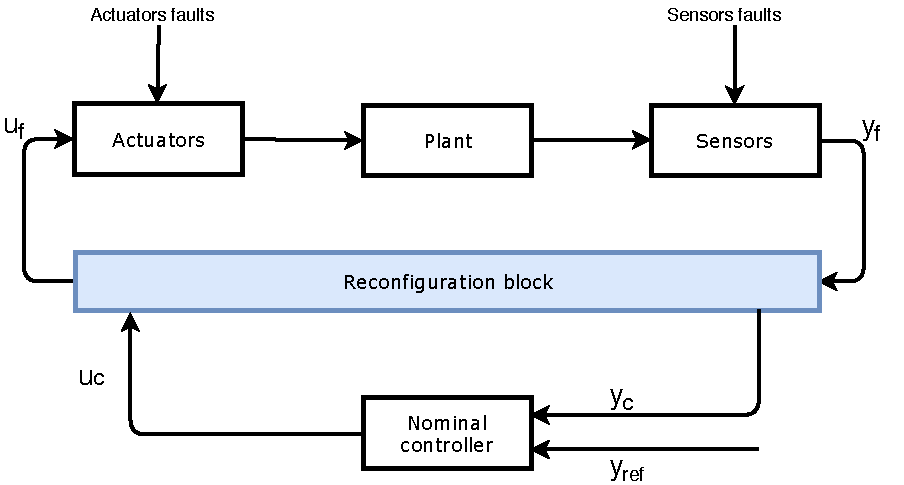
\includegraphics[width=0.8\linewidth]{figures/VirtualActuator}
	\caption{ Virtual actuators and sensors scheme}
	\label{fig:VA}
\end{figure}

If that the main controller remain unchanged, a reconfiguration between the system and the output of the controller is made. If a fault in the actuators or sensors will occur, then the reconfiguration block has the possibility to give as an output a signal that is similar with the one that the actuator or sensor will have for the nominal controller.

In the case that a fault will occur in the reaction wheel sensor, the angular velocity measurement it is assumed functional and based on that measurement, the torque output form the faulty wheel can be computed. A second assumption is that the sensors will completely fail, but in this case a model of how the angular velocity of the wheel is decreasing over time is obtained. This model can be used as a virtual sensor for the angular velocity sensor. 
